迄今为止，我们研究的统计问题都围绕最优传输距离及其变体的估计展开. 然而，在最优传输的多种应用中——仅举数例，包括数据融合（data fusion）\cite{ref93}、适应／迁移学习（adaptation/transfer learning）\cite{ref94}和计算生物学（computational biology）\cite{ref58,ref283}——主要关注的对象是最优传输映射. 本章讨论如何根据有限个样本估计这一映射.

\subsection{问题表述}\label{sec:3.1}
回顾 Brenier 定理：如果 $\mu$ 有密度，则
$$
\begin{aligned}
W_2^2(\mu,\nu)&=\min_{\gamma\in\Gamma_{\mu,\nu}}\int\|x-y\|^2\,\gamma(dx,dy)\\
&=\min_{T:T_\#\mu=\nu}\int\|x-T(x)\|^2\,\mu(dx).
\end{aligned}
$$
此外，最优传输映射具有 $T=\nabla\varphi$ 的形式，其中 $\varphi$ 为凸函数. 也可以写成 $(X,\nabla\varphi(X))\sim\gamma$，或者 $\gamma(dx,dy)=\mu(dx)\delta_{T(x)}(dy)$.

要研究的统计问题表述如下：给定样本 $X_1,\ldots,X_n\overset{\mathrm{i.i.d.}}\sim\mu$ 和 $Y_1,\ldots,Y_n\overset{\mathrm{i.i.d.}}\sim\nu$，如何利用根据这些样本构造的估计量 $\widehat T$，来估计从 $\mu$ 到 $\nu$ 的最优传输映射 $T$？

我们采用积分误差（integrated error）作为性能度量：
$$\int\|\widehat T(x)-T(x)\|^2\,\mu(dx).$$

\begin{figure}[htbp]\centering
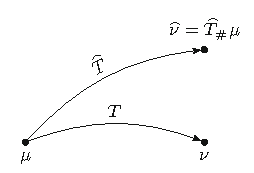
\includegraphics[width=0.29\textwidth]{assets/chapter3/figure-3-1.pdf}
\caption{传输映射之间的 $L^2$ 误差控制 $\widehat\nu$ 与 $\nu$ 之间的 $W_2^2$ 距离.}\label{fig:3.1}
\end{figure}
\begin{figure}[htbp]\centering
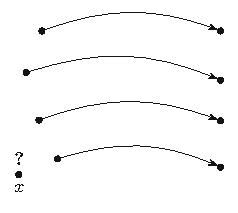
\includegraphics[width=0.28\textwidth]{assets/chapter3/figure-3-2.pdf}
\caption{如何在样本外的点 $x$ 处对经验最优传输映射作插值？}\label{fig:3.2}
\end{figure}

$L^2$ 积分误差是非参数统计中常用的一种自然距离度量. 不过，在这里它还有另一层解释：控制 $\mu$ 在两个映射下的推前测度之间的 Wasserstein 距离. 更准确地说，根据定义 $\nu=T_\#\mu$. 如果通过 $\widehat\nu=\widehat T_\#\mu$ 定义测度 $\widehat\nu$，那么对于 $X\sim\mu$，$(\widehat T(X),T(X))$ 是 $\widehat\nu$ 与 $\nu$ 的一个次优耦合，因而
$$
W_2^2(\widehat\nu,\nu)\le\mathbb E\|\widehat T(X)-T(X)\|^2
=\int\|\widehat T(x)-T(x)\|^2\,\mu(dx).
$$
示意见\autoref{fig:3.1}.

一种初步的估计方法可能是计算经验测度 $\mu_n$ 与 $\nu_n$ 之间的最优耦合，即求解 $\min_{\gamma\in\Gamma_{\mu_n,\nu_n}}\int\|x-y\|^2\,\gamma(dx,dy)$，但我们很快就会发现这一朴素方案存在一个无法回避的缺口. 即使最优传输计划 $\gamma_n$ 由某个传输映射 $T_n$ 诱导，从而 $\gamma_n(dx,dy)=\mu_n(dx)\delta_{T_n(x)}(dy)$，映射 $T_n$ 也仅在样本 $\{X_1,\ldots,X_n\}$ 上有良好定义，尚不清楚如何有原则地将其延拓为整个 $\mathbb R^d$ 上的映射（\autoref{fig:3.2}）. 为解决这一问题，文献中提出了多种方法，旨在构造 $T_n$ 到样本外各点的插值 $\widehat T_n$. 例如，可以令 $\widehat T_n(x)=T_n(X_i)$，其中 $X_i$ 是距离 $x$ 最近的样本点. 这就是 1-最近邻估计量（1-nearest neighbor estimator）；可以证明，在没有额外光滑性假设时，它具有极小极大最优性\cite{ref221}；一维情形见\autoref{exer:3.1}. 不过，这种方法无法利用 $\mu$ 和 $\nu$ 的额外正则性，我们在此不再继续讨论.

相反，下一节将根据最优传输的半对偶表述设计一个估计量. 这一估计策略的优点在于，能够灵活纳入对总体传输映射 $T$ 的额外假设，例如光滑性. 采用足够强的假设，就可以得到避开维数灾难的映射估计量.
